\chapter{Design and Implementation}


The chapter introduces core design decisions in terms of components, data structures and algorithms. It also discuses the reasoning behind choices made, alternatives and tradeofs.


% -----------------------
\section{Tree Structures}

% requirements, alternatives, choices
For the most part of the wrapping process, the core data structure that is being manipulated is a labeled ordered tree. The algorithms used require a small number of (mostly navigation) operations on trees. While there are certainly a great number of various graph libraries, most of them add extra level of complexity in terms of unnecessary operations and unused data stored. Thus, we decided to implement a light-weight tree data structure on our own.

% class diagram
\begin{figure}[h]
	\centering
	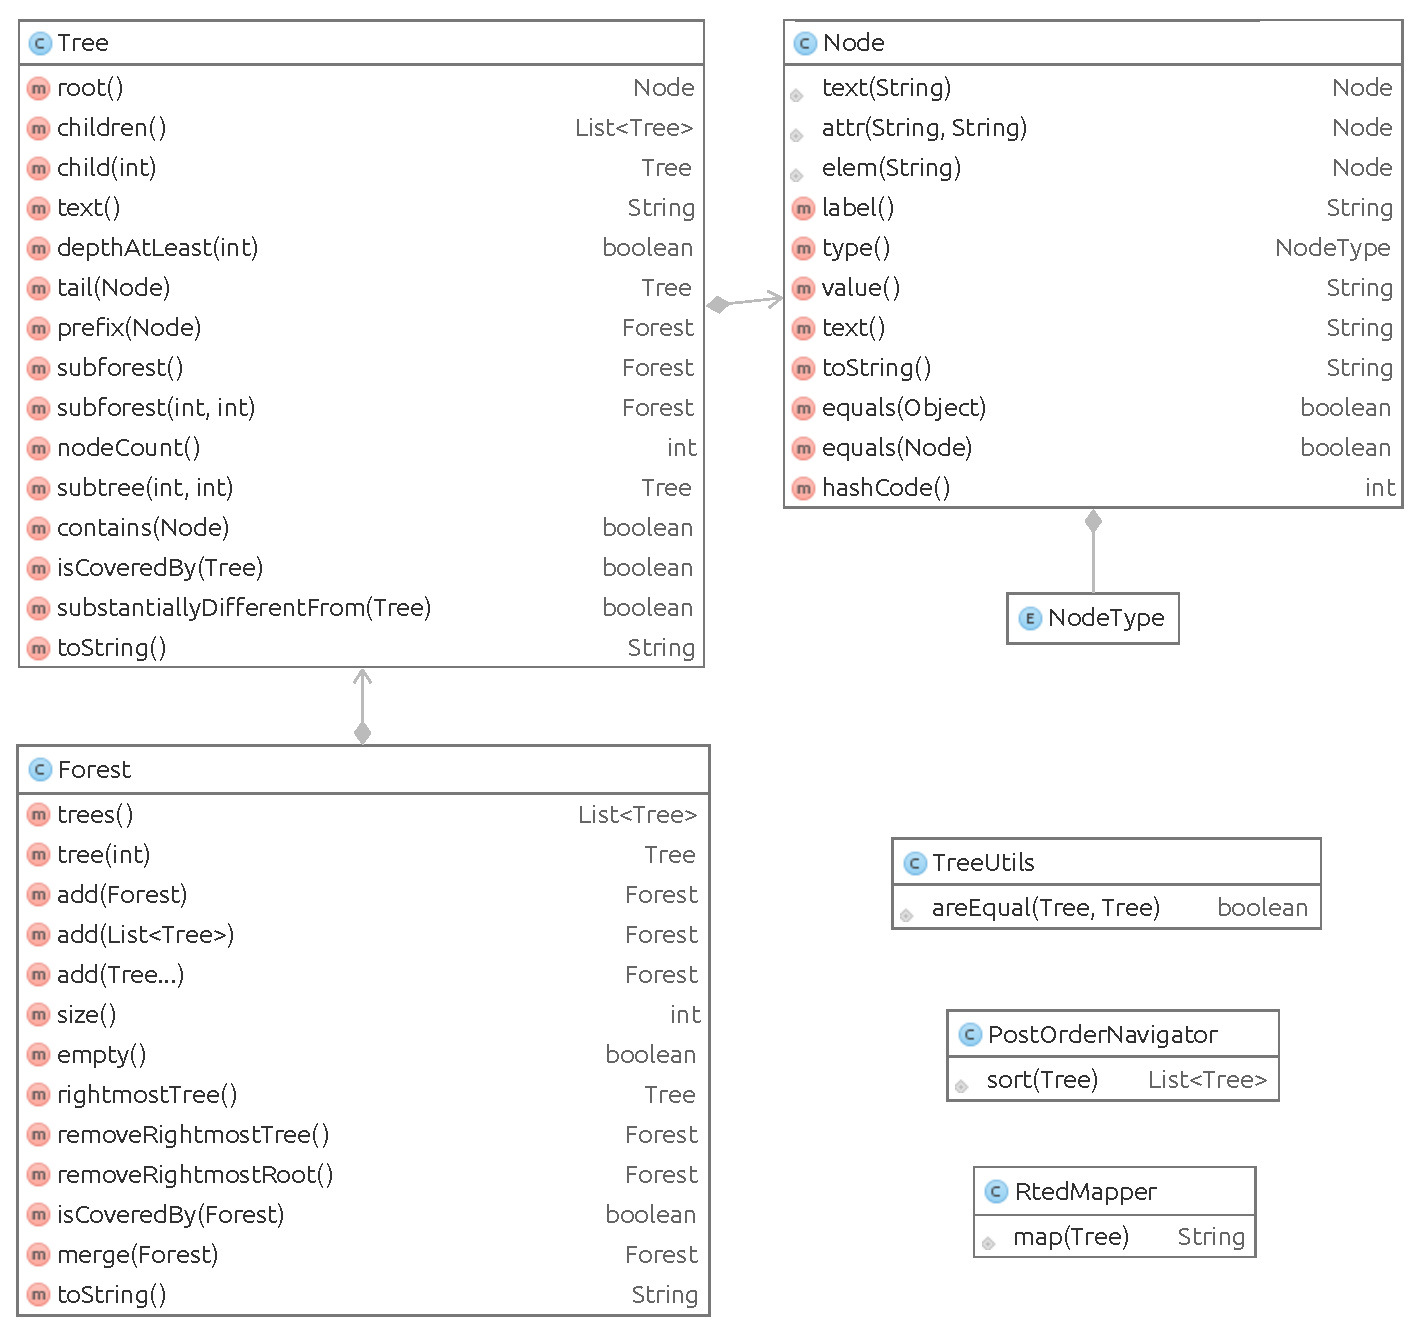
\includegraphics[width=1.0\textwidth]{figures/package-tree}
	\caption{Tree package class diagram.}
	\label{fig:package-tree}
\end{figure}

% entities
There are three essential classes that represent a graph (see Figure~\ref{fig:package-tree}). The actual data is stored in a \texttt{Node}. A \texttt{Tree} organizes the \texttt{Node} objects into a hierarchical structure with a root node. A \texttt{Forest} combines a set of \texttt{Tree} objects to represent a disjoint union of trees. All classes are immutable, which allows for further data manipulation without the state management problems.

% behaviour for each entity

\paragraph{Node} As we primarily aim at wrapping HTML documents, we build a tree of three types of \texttt{Node} objects: an element, an attribute or a text. The class has a convenience factory methods for building a \texttt{Node} of each type.

\paragraph{Tree} The \texttt{Tree} class stores current root node and a pointer to each of its subtrees. The class enables to select different parts of the tree for many of its use cases: \texttt{children()}, \texttt{child()}, \texttt{tail()}, \texttt{prefix()}, \texttt{subforest()}, \texttt{subtree()}. Due to its hierarchical structure, the most of methods in the class are recursive. A tree comparison heuristics is implemented in \texttt{substantiallyDifferentFrom()} method, which compares the node count of two trees.

\paragraph{Forest} Some operations on trees, e.g. \texttt{tail()}, return a disjoint set of trees. These are grouped under a \texttt{Forest} class. It also adds convinience methods for manipulating the forest: \texttt{removeRightmostTree()} and \texttt{removeRightmostRoot()}. It is important to note that the data structure is immutable, and all edit oprations return a new instance of a \texttt{Forest}. This helps to avoid state management.

\paragraph{TreeUtils} Tree structure comparison is extracted as an utility method in \texttt{TreeUtils} class. This approach was chosen over \texttt{equals()} method inside the \texttt{Tree} class, in order not to break a key inside key-value collections through \texttt{hashCode()} method.

\paragraph{PostOrderNavigator} \texttt{PostOrderNavigator} walks the tree in a post-order and returns a list of visited nodes.

\paragraph{RtedMapper} For tree edit-distance calculations we use RTED library from \cite{pawlik2011a}. The library uses a string representation of trees as input. Thus we use adapter \texttt{RtedMapper} to map our \texttt{Tree} object into the required string.


% ---------------------------
\section{Data Region Locator}

% requirements, alternatives, choices

% class diagram
\begin{figure}[h]
	\centering
	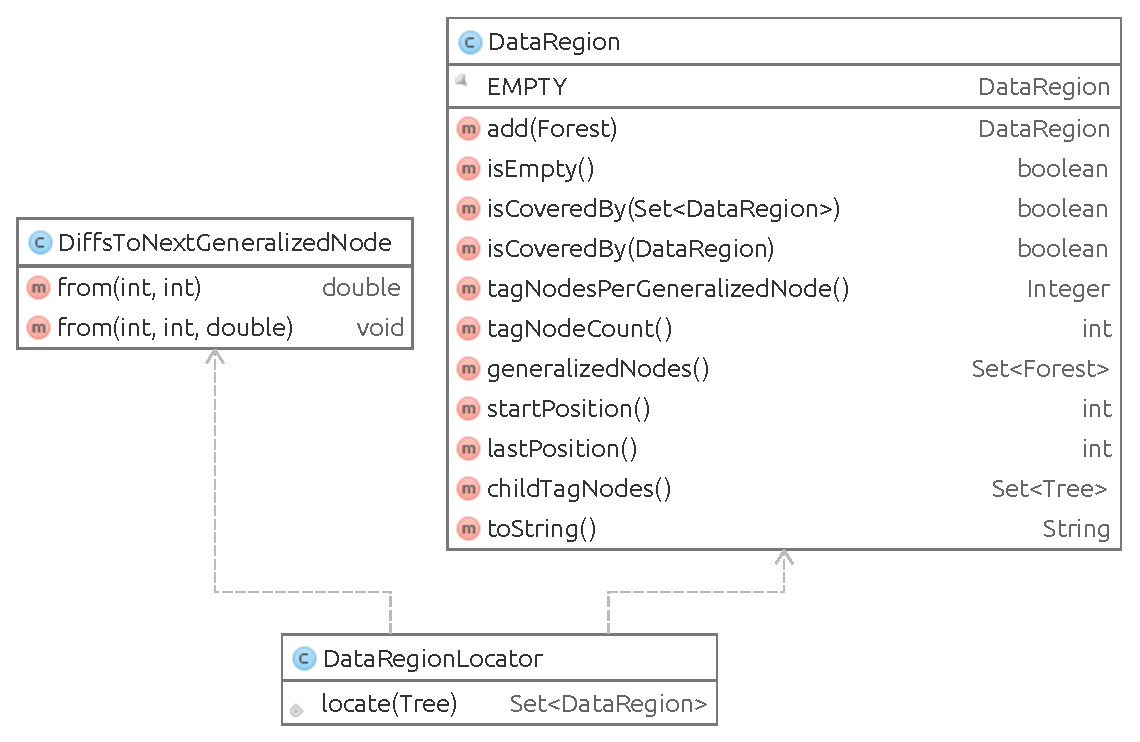
\includegraphics[width=1.0\textwidth]{figures/package-region}
	\caption{Region package class diagram.}
	\label{fig:package-region}
\end{figure}

% entities
Data region locator logic is grouped in the \texttt{region} package (see Figure~\ref{fig:package-region}). \texttt{DataRegion} class contains the data record structure, while \texttt{DataRegionLocator} implements the Algorithm~\ref{alg:locating-data-region-containing-node} for locating data regions. \texttt{DiffsToNextGeneralizedNode} is data structure for convenient storage of tree edit-distances.

% behaviour for each entity

\paragraph{DataRegion} The \texttt{DataRegion} class contains a set of data records (i.e. \texttt{Forest} classes) and a position index from its parent node in a tree. The method \texttt{isCoveredBy()} checks whether two data regions overlap. The other methods are getters for accessing various pieces of data records.

\paragraph{DataRegionLocator} The \texttt{DataRegionLocator} logic is split across three private methods: \texttt{calcCombinations()}, \texttt{findDataRegions()}, and \texttt{identifyDataRecords()}. These basically implement the Algorithm~\ref{alg:locating-data-region-containing-node} directly. Yet there are a few custom heuristics and optimizations. First, we limit a number of nodes per data record to 3 to reduce the search space. Next, we limit edit-distance calculations for trees that are not substantially different. Finally, we use RTED library from \cite{pawlik2011a} to compute tree edit-distance instead of Lavenshtein distance for string edit-distance.

\paragraph{DiffsToNextGeneralizedNode} The \texttt{DiffsToNextGeneralizedNode} is a convenience data structure for two dimensional array access.


% --------------------
\section{Change Model}

% requirements, alternatives, choices
This package (see Figure~\ref{fig:package-changemodel}) contains the probabilistic transducer \emph{TP} and a change model from Algorithm~\ref{alg:prob-record-level-wrapper} described by Dalvi et al. \cite{dalvi2009a}. The implementation follows a recursive algorithm nature as defined by Dalvi. 

We don't learn a probabilistic model of change from web page archive. We assume it is provided. We consider that having a universal HTML change model is in line with Dalvi et al. \cite{dalvi2009a} findings, that models learned on two different datasets were quite similar without major differences.

% class diagram
\begin{figure}[h]
	\centering
	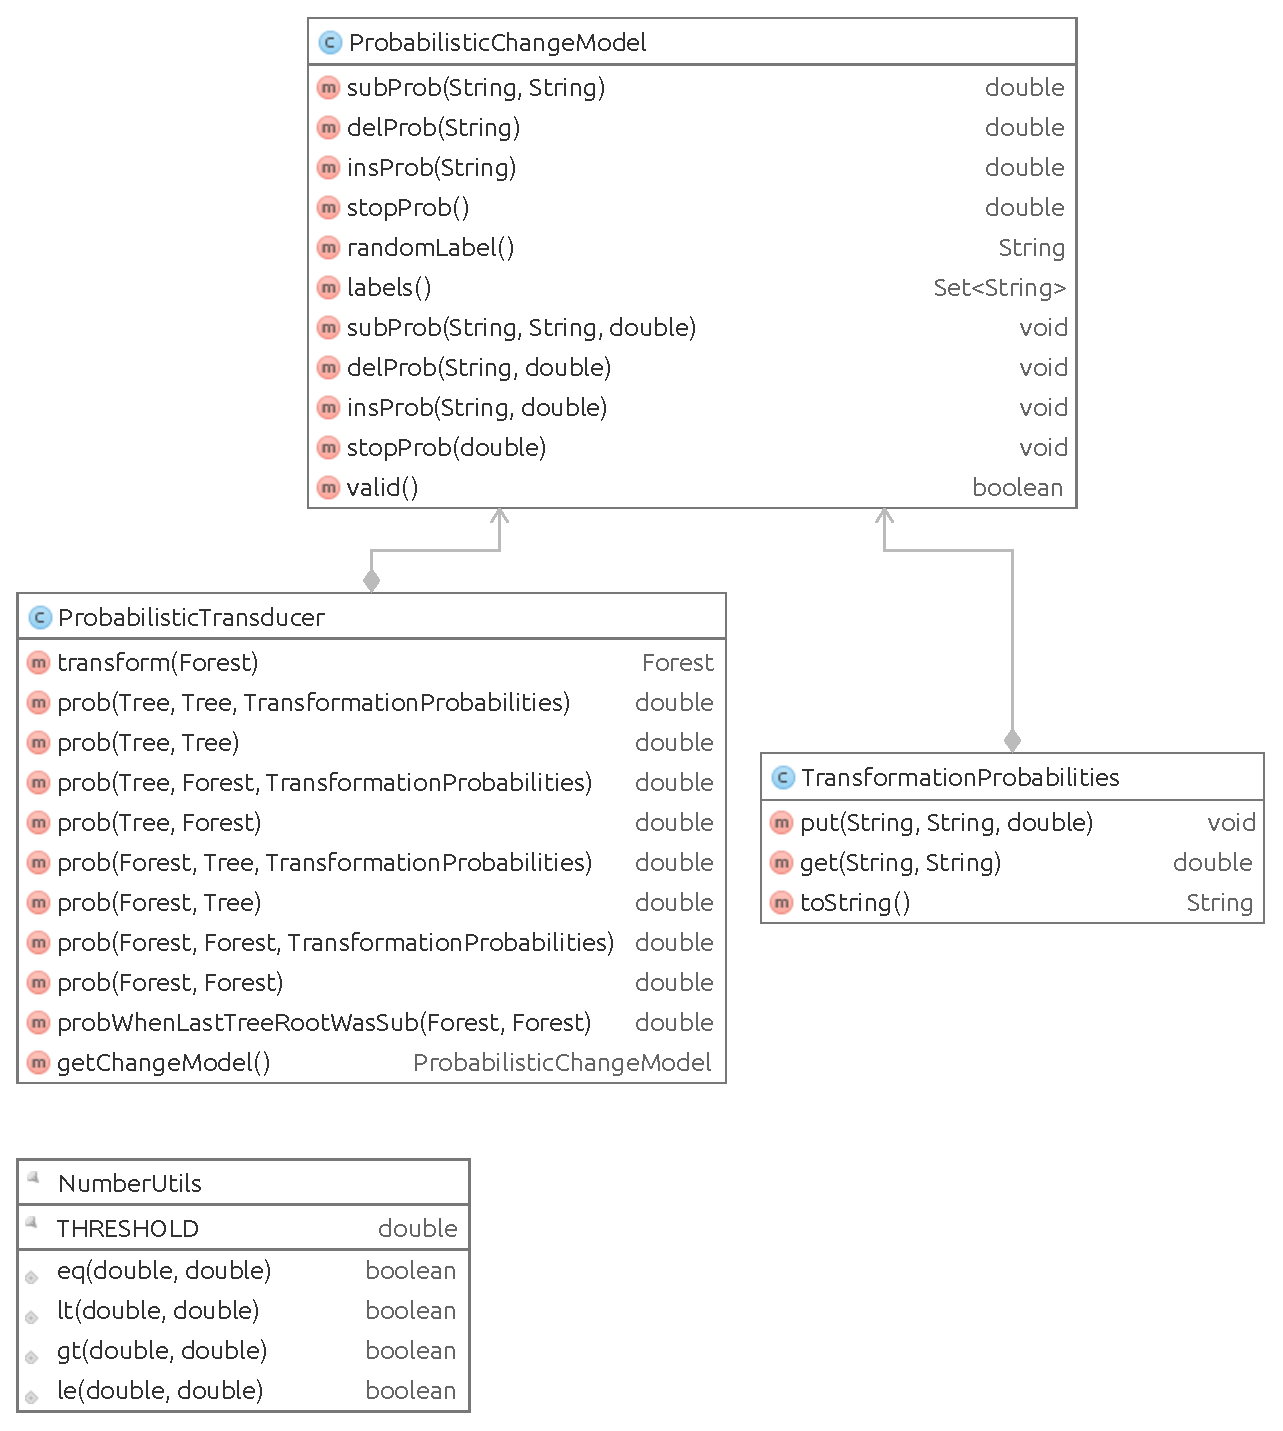
\includegraphics[width=1.0\textwidth]{figures/package-changemodel}
	\caption{Change Model package class diagram.}
	\label{fig:package-changemodel}
\end{figure}

% entities
The core logic is in the \texttt{ProbabilisticTransducer} class. The probabilities of HTML tag modification is stored in a \texttt{ProbabilisticChangeModel} data structure. \texttt{TransformationProbabilities} class acts as a cache to store transformation probabilities for trees. \texttt{NumberUtils} is a helper class for floatating point calculations.

% behaviour for each entity

\paragraph{ProbabilisticChangeModel} The class \texttt{ProbabilisticChangeModel} is a data structure for storing insert, delete and substitute probabilities of various HTML tags. It contains getters and setters for probabilities. The method \texttt{valid()} checks, if sum of all probabilities is $1.0$ and other rules hold. This is helpful for validating data input, as change models are loaded but not learned by our implementation.

\paragraph{TransformationProbabilities} After calculating the chance of one tree being transformed into another tree, we store the probability in a cache, i.e. \texttt{TransformationProbabilities} class. This class acts as an in-memory key-value storage. By caching the probabilities, we reduce the amount of caculation in recursive $TP$ calls in Algorith~\ref{alg:prob-record-level-wrapper}.

\paragraph{ProbabilisticTransducer} The class \texttt{ProbabilisticTransducer} calculates a probability of transforming original tree into transformed one in \texttt{prob()} method. The method is provided with a number of convenience interfaces. The implementation adds a performance optimization for substantially different trees and a caching strategy for repeat tree comparison.

The class also provides a random process \texttt{transform()}, that makes one pass over the whole forest and at each position, it randomly decides to either delete a node, change its label, or insert new nodes.

\paragraph{NumberUtils} As probabilities are stored in a floating point numbers, the use of class \texttt{NumberUtils} ensures 6 digit decimal point precision.


% ------------------------------
\section{Probabilistic Wrappers}

% requirements, alternatives, choices

% class diagram
\begin{figure}[h]
	\centering
	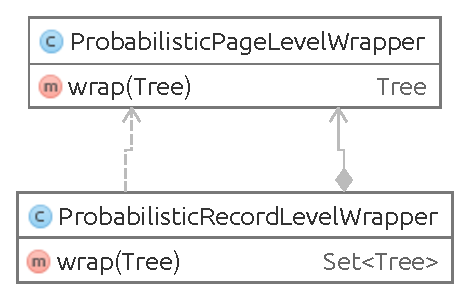
\includegraphics[width=0.33\textwidth]{figures/package-wrapper}
	\caption{Wrapper package class diagram.}
	\label{fig:package-wrapper}
\end{figure}

% entities

% behaviour for each entity

\paragraph{ProbabilisticPageLevelWrapper}

\paragraph{ProbabilisticRecordLevelWrapper}


% ----------------------------
\section{HTML Document Parser}

% requirements, alternatives, choices

% class diagram
\begin{figure}[h]
	\centering
	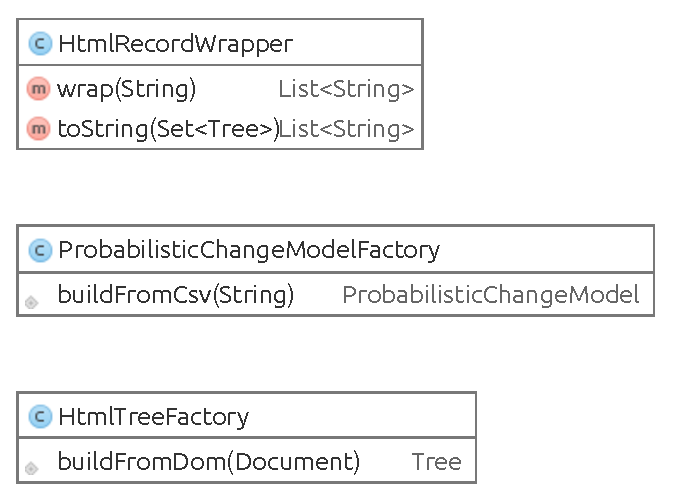
\includegraphics[width=0.5\textwidth]{figures/package-html}
	\caption{HTML package class diagram.}
	\label{fig:package-html}
\end{figure}

% entities

% behaviour for each entity

\paragraph{HtmlRecordWrapper}

\paragraph{ProbabilisticChangeModelFactory}

\paragraph{HtmlTreeFactory}


% vim:wrap linebreak nolist:
